% ASSIGNMENT 3 SPECTRAL ESTIMATION AND MODELLING

\section{Spectral Estimation and Modelling}

\lhead{Advanced Signal Processing}
\rhead{Spectral Estimation and Modelling}

The PSD of an ergodic stochastic process \boldsymbol{X_{n}} is the power distribution of its constituent frequency components. The PSD can be approximated by a signal known as the periodogram which is calculated using the FFT algorithm as in Equation \ref{eqn:periodogram}.

\begin{equation}
\hat{P}_{X}(f)=\frac{1}{N}\left|\sum_{n=0}^{N-1} x[n] e^{\frac{-j f n 2 \pi}{N}}\right|^{2}
\label{eqn:periodogram}
\end{equation}
\noindent
where $f$ = frequency, $n$ = sample number and $N$ = total number of samples.
\\\\
I implemented this algorithm in a MATLAB function named \code{pgm.m} which is shown below.
\\\\
\noindent
\code{
\textcolor{blue}{function} [pgm\_out] = pgm(x)
\\\textcolor{white}{....}N = length(x);
\\\textcolor{white}{....}pgm\_out = (1/N)*abs(fft(x)).\string^2;
\\\textcolor{blue}{end}
}
\\\\
\noindent
This function was applied to WGN processes of lengths N = 128, 256, and 512 obtaining the results shown in Figure \ref{fig:pgms}. The x-axis was also manually rescaled to show zero-center the periodograms and show normalised frequency.

\begin{figure}[H]
\begin{subfigure}{.32\textwidth}
  \centering
  \includegraphics[width=\linewidth]{assignment3figs/pgm_128.eps}  
  \caption{Data length N = 128.}
\end{subfigure}
\begin{subfigure}{.32\textwidth}
  \centering
  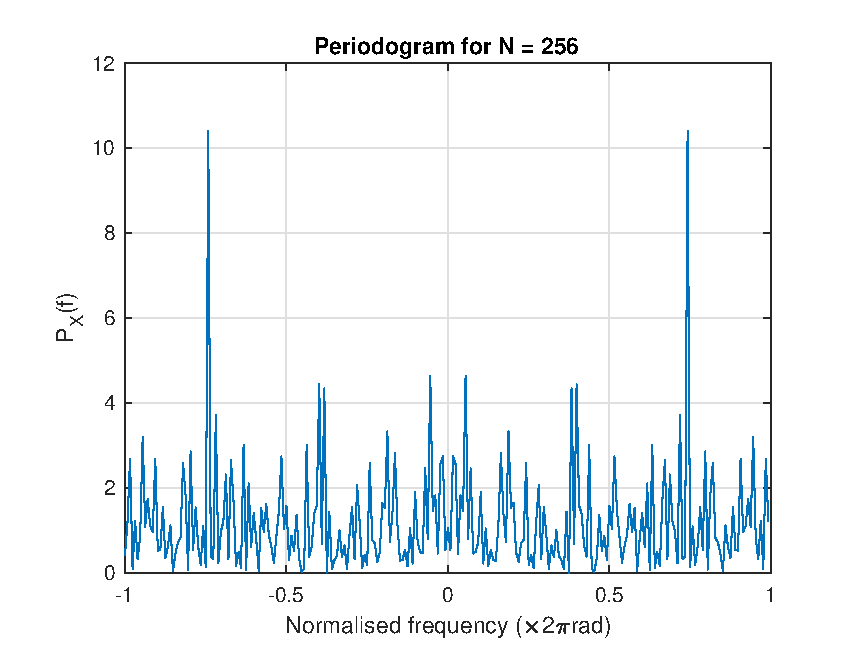
\includegraphics[width=\linewidth]{assignment3figs/pgm_256.eps}  
  \caption{Data length N = 256.}
\end{subfigure}
\begin{subfigure}{.32\textwidth}
  \centering
  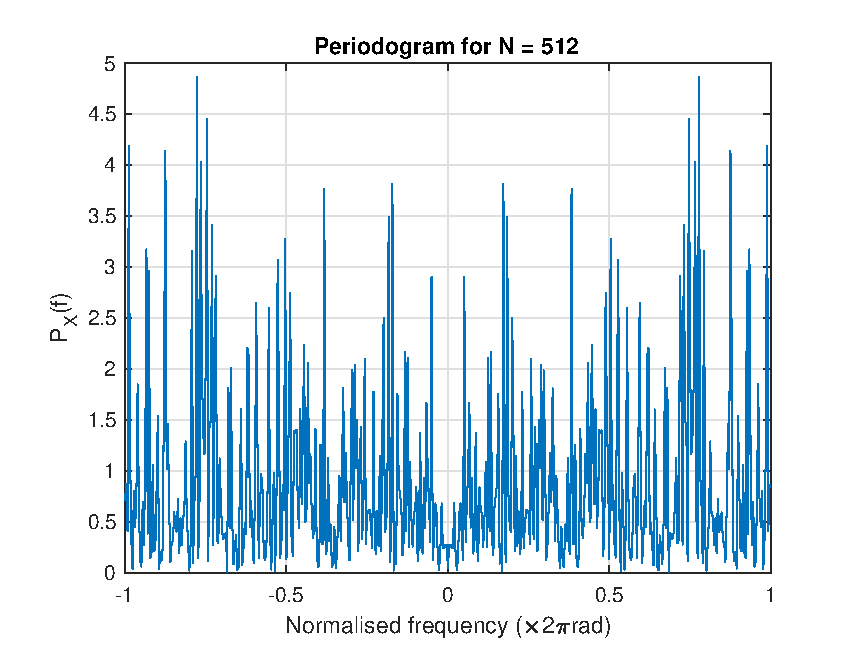
\includegraphics[width=\linewidth]{assignment3figs/pgm_512.eps}  
  \caption{Data length N = 512.}
\end{subfigure}
\caption{Periodograms for WGN processes of variable lengths.}
\label{fig:pgms}
\end{figure}

\noindent
By rescaling the axis, the expected symmetry of the periodogram becomes evident. The ideal PSD would be 1 for all frequencies since a defining feature WGN is that it is 'white', meaning that it contains all frequencies in equal proportions. Whilst the periodograms do not match this, the mean does appear to be roughly 1, which agrees with our expectations. 

% 3.1 Averaged periodogram estimates
\subsection{Averaged periodogram estimates}

\subsubsection{Smoothing periodograms}

Applying a zero-phase FIR filter to the periodogram has a smoothing effect. A filter with the impulse response h = [0.2 0.2 0.2 0.2 0.2] was applied to the periodograms. The results are shown in Figure \ref{fig:pgms_filt}.

\begin{figure}[H]
\begin{subfigure}{.32\textwidth}
  \centering
  \includegraphics[width=\linewidth]{assignment3figs/pgm_filt128.eps}  
  \caption{Data length N = 128.}
\end{subfigure}
\begin{subfigure}{.32\textwidth}
  \centering
  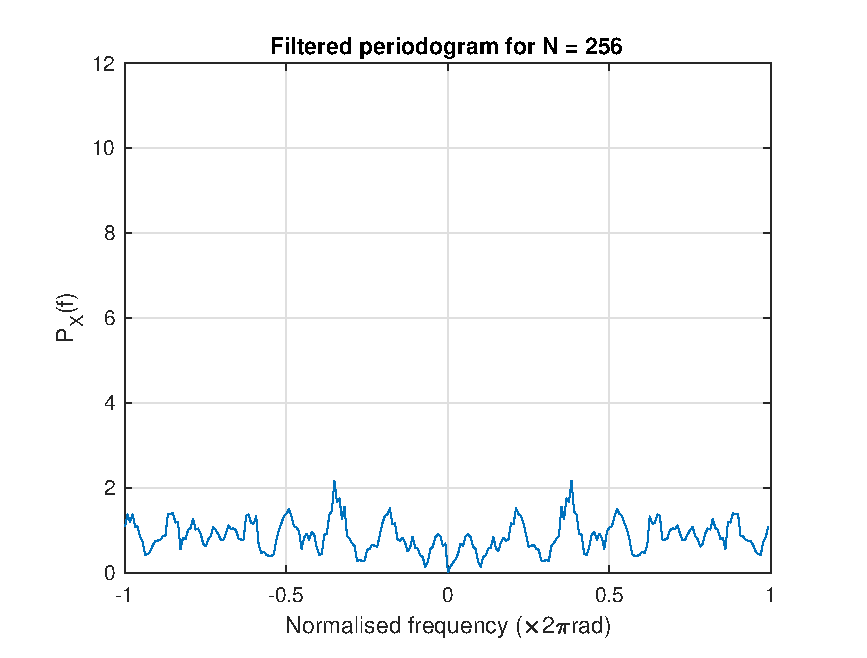
\includegraphics[width=\linewidth]{assignment3figs/pgm_filt256.eps}  
  \caption{Data length N = 256.}
\end{subfigure}
\begin{subfigure}{.32\textwidth}
  \centering
  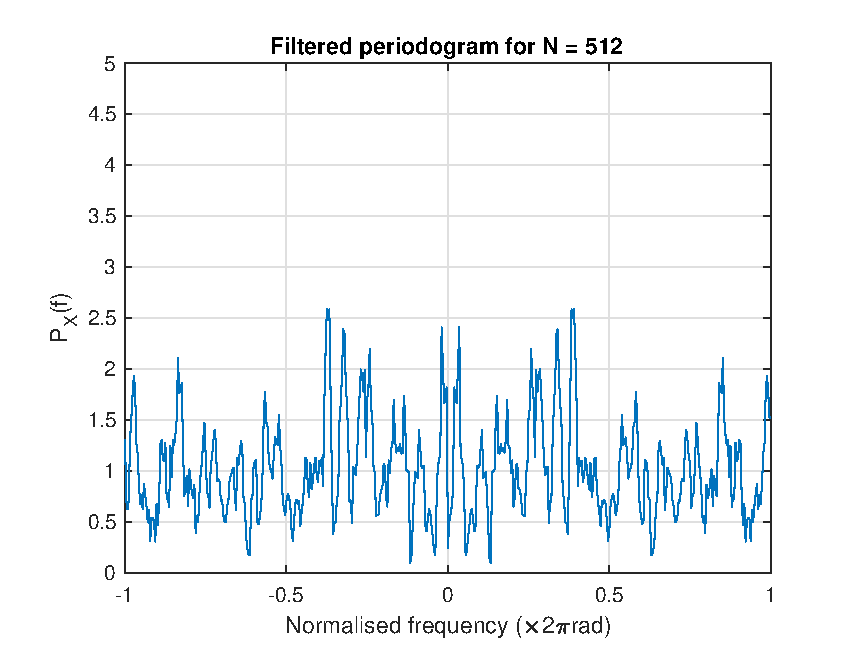
\includegraphics[width=\linewidth]{assignment3figs/pgm_filt512.eps}  
  \caption{Data length N = 512.}
\end{subfigure}
\caption{Filtered periodograms for WGN processes of variable lengths with same axis scale.}
\label{fig:pgms_filt}
\end{figure}

\noindent
Comparing the plots in Figure \ref{fig:pgms_filt} with those in Figure \ref{fig:pgms}, the smoothing effect of the applied filter is evident. By filtering out higher frequencies, it enables us to see the general shape of the signals and thus they more interpretable than the unfiltered versions.


\subsubsection{Periodograms of non-overlapping segments}

The 1024-sample WGN signal was divided into 8 128-sample segments whose periodograms were obtained using the \code{pgm.m} function. The results are shown in Figure \ref{fig:pgms_compound}.

\begin{figure}[H]
    \centering
    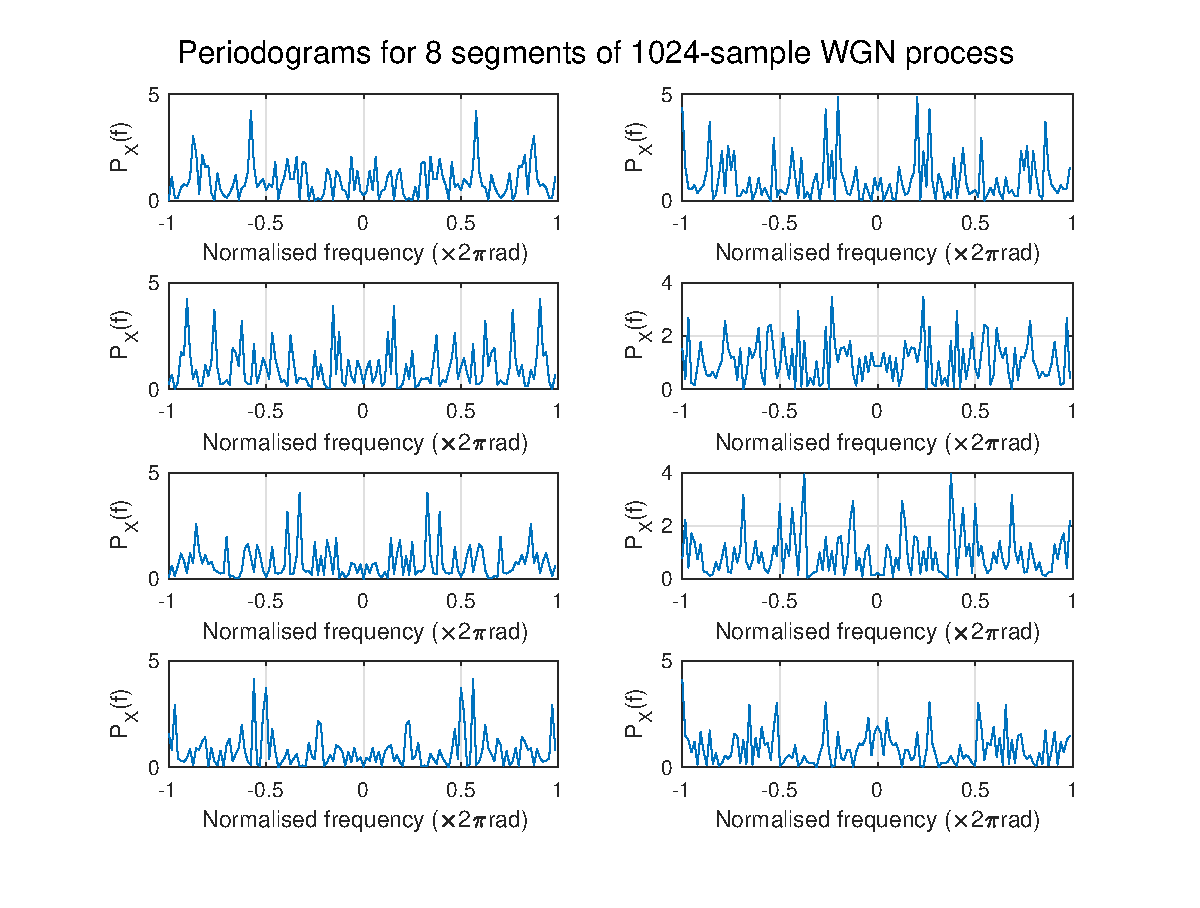
\includegraphics[width=16cm]{assignment3figs/pgms_compound.eps}
    \caption{Periodograms obtained for 8 segments of WGN process}
    \label{fig:pgms_compound}
\end{figure}

\noindent
These periodograms appear to have the same effect as generating individual 128-sample WGN processes. This can be explained by the fact that WGN is a stationary process, therefore the mean and variance are constant in time so the theoretical PSD of any given segment is the same.

\subsubsection{Average periodogram}

The 8 periodograms in Figure \ref{fig:pgms_compound} were averaged using MATLAB's \code{mean()} function to obtain an average periodogram, which is shown in Figure \ref{fig:avg_pgm}.

\begin{figure}[H]
    \centering
    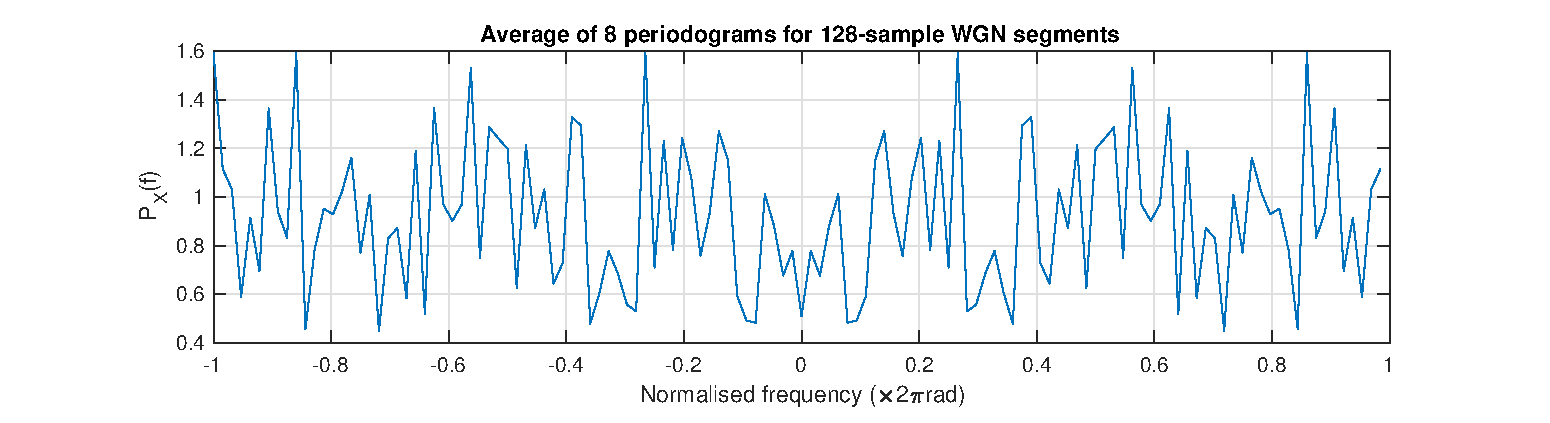
\includegraphics[width=13cm]{assignment3figs/avg_pgm.eps}
    \caption{Average periodogram obtained from 8 segments.}
    \label{fig:avg_pgm}
\end{figure}

\noindent
In this averaged periodogram, the variance of the signal is significantly lower and the signal mean of 1 is much more clear. This is because averaging has the effect of making the statistical properties of the process clearer as the signal tends towards the ideal theoretical PSD (which, as previously mentioned, is constant at 1). This implies that averaging the periodogram across segments provides a better estimate than generating a single periodogram.

% 3.2 Spectrum of autoregressive processes
\subsection{Spectrum of autoregressive processes}

A 1024-sample WGN signal was generated and subsequently filtered using MATLAB's \code{filter()} function. The filter used has the transfer function given by Equation \ref{eqn:filt1}.

\begin{equation}
    H(z) = \frac{1}{1+0.9e^{-z}}
    \label{eqn:filt1}
\end{equation}

\noindent
The effect of filtering is shown in Figure \ref{fig:filtering}.

\begin{figure}[H]
    \centering
    \subfloat[Unfiltered.]{{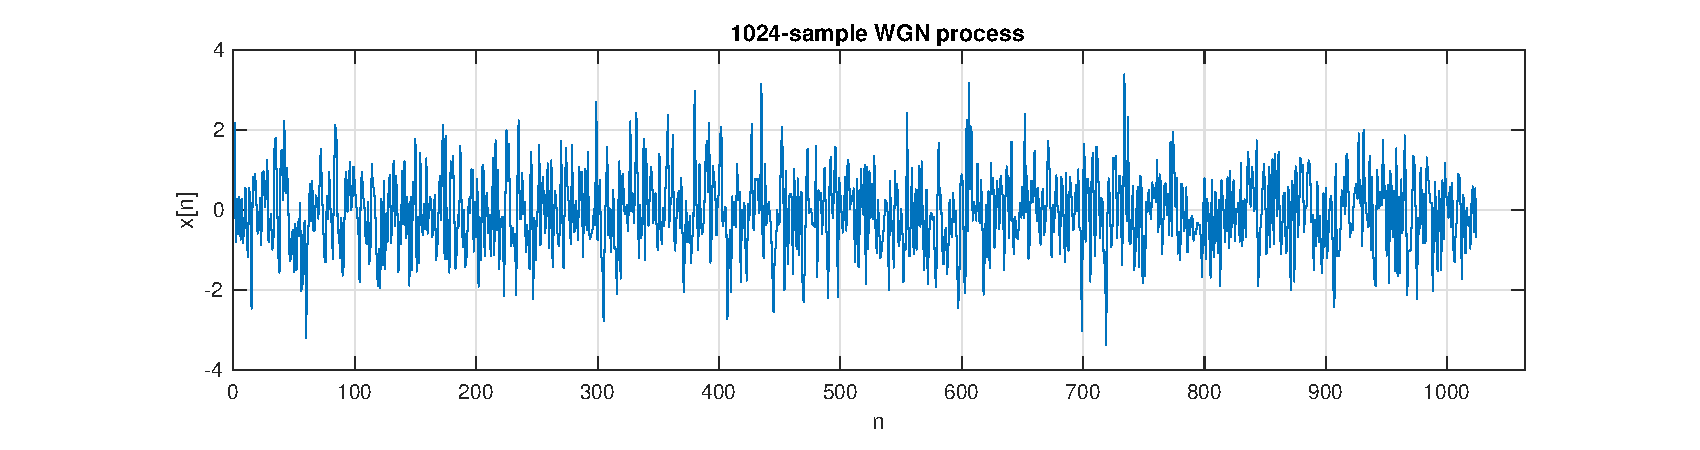
\includegraphics[width=13cm]{assignment3figs/1024_unfilt.eps}}}\\
    \subfloat[Filtered.]{{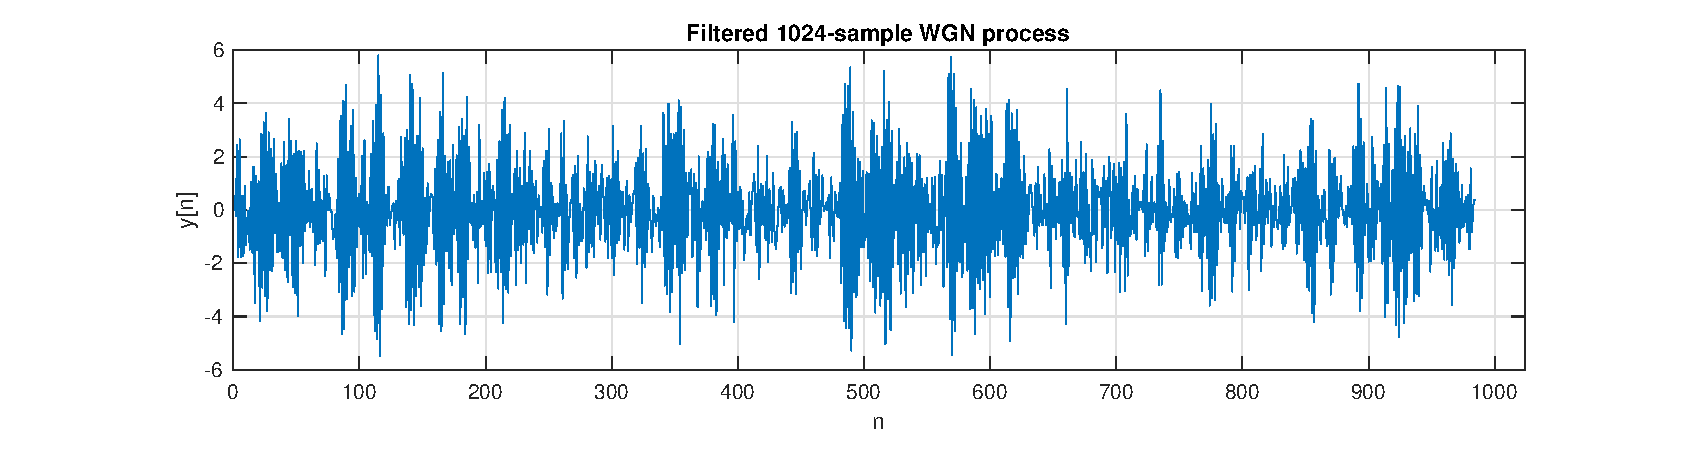
\includegraphics[width=13cm]{assignment3figs/1024_filt.eps}}}
    \caption{Effect of filtering on WGN process.}
    \label{fig:filtering}
\end{figure}

\noindent
Filtering clearly has the effect of increasing the variance of the signal. The signal also appears to have more high frequency oscillations, and has acted as a HPF.

\subsubsection{The periodogram and the PSD}

\noindent
The PSD can be calculated using Equation \ref{eqn:psdeqn}.

\begin{equation}
P_{Y}(f)=\frac{\sigma_{X}^{2}}{\left|1+\sum_{k=1}^{p} a_{k} e^{-j 2 k h \pi}\right|^{2}} 
\label{eqn:psdeqn}
\end{equation}

\noindent
This equation was applied to the WGN process in question, obtaining the result shown in Figure \ref{fig:idealpsd}.

\begin{figure}[H]
    \centering
    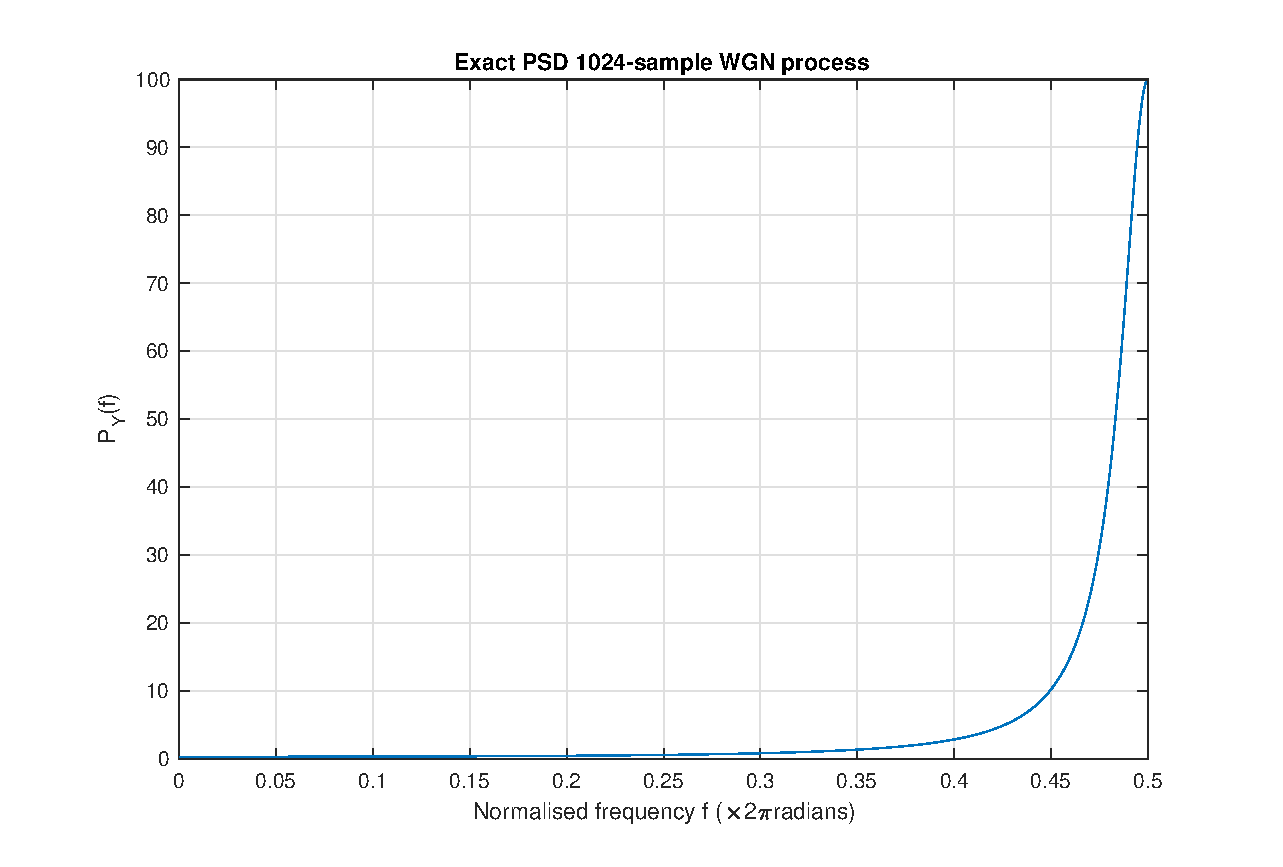
\includegraphics[width=7cm]{assignment3figs/ideal_psd.eps}
    \caption{Ideal PSD calculated using Equation \ref{eqn:psdeqn}.}
    \label{fig:idealpsd}
\end{figure}

\noindent
Subsequently, the \code{pgm.m} function was used to approximate the PSD with a periodogram. The comparison of these is shown in Figure \ref{fig:pgmandzoom}.

\begin{figure}[H]
    \centering
    \subfloat[PSD vs periodogram.]{{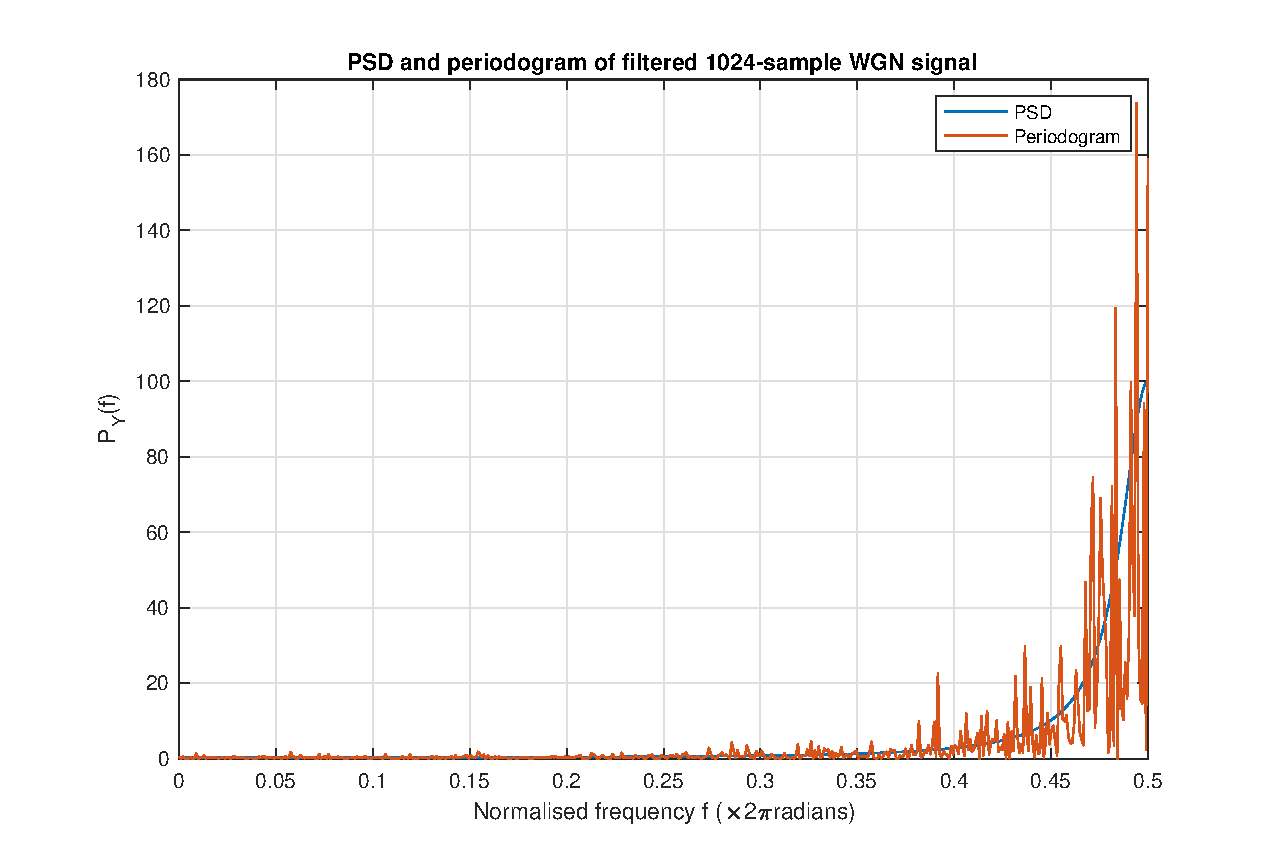
\includegraphics[width=7cm]{assignment3figs/pgm_psd.eps}}}
    \subfloat[Zooming in on high frequencies.]{{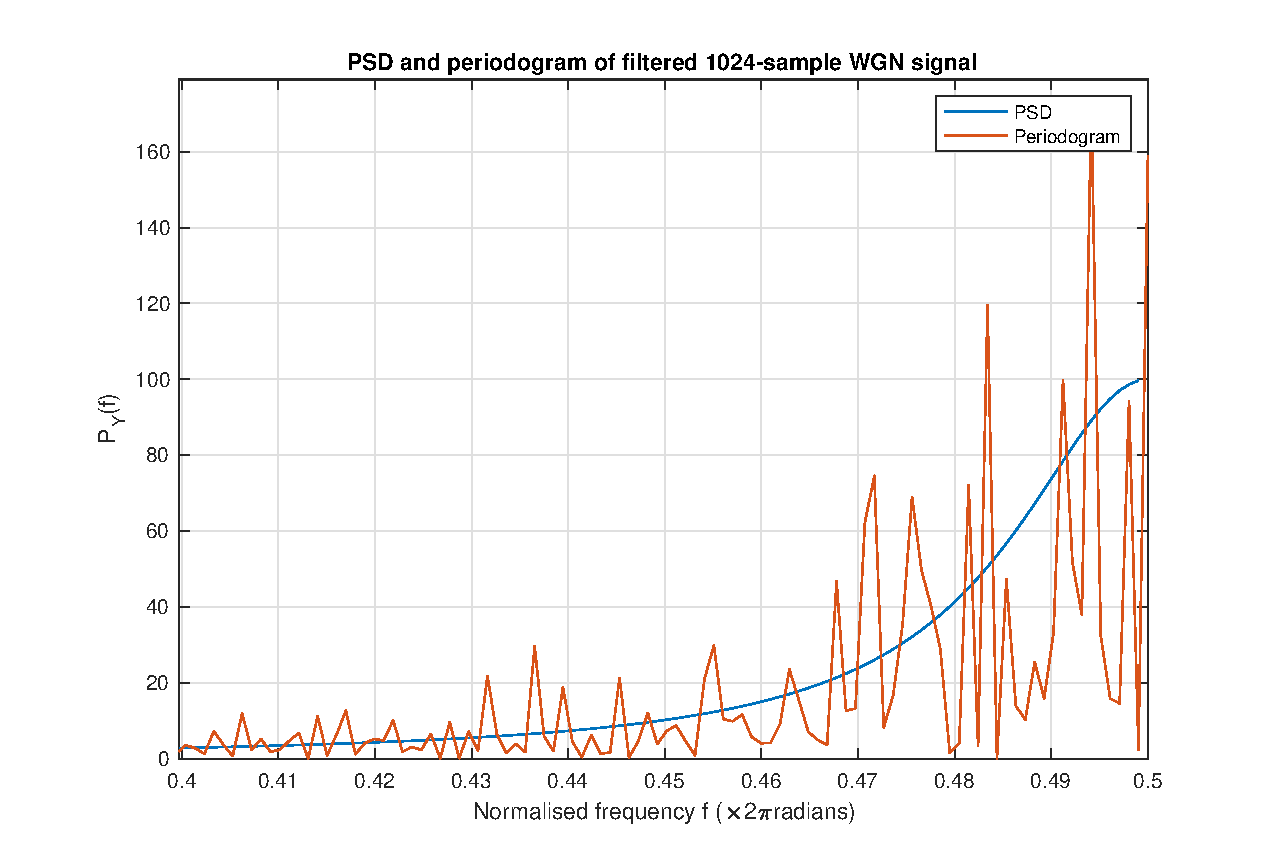
\includegraphics[width=7cm]{assignment3figs/pgm_psd_zoom.eps}}}
    \caption{Comparison of PSD and periodogram.}
    \label{fig:pgmandzoom}
\end{figure}

\noindent
From Figure \ref{fig:pgmandzoom}a, the periodogram appears to be a reasonable approximation of the PSD, since the signal power is concentrated at higher frequencies and the periodogram follows the same shape as the PSD. Figure \ref{fig:pgmandzoom}b zooms in on (a) for frequencies between 0.4Hz and 0.5 Hz. It is evident from this that, despite following the same general shape as the PSD, the periodogram oscillated with increasing variance. This arises due to the fact that the periodogram is generated using a rectangular window function at each time instant. In the frequency domain, multiplication with a rectangular window is equivalent to convolution with a sinc() function (when the sampling frequency is above the Nyquist-frequency). The resultant signal is therefore oscillatory. The signal could be smoothed by averaging across periodograms of segments of the original signal, reducing the variance of the signal and better approximating the ideal PSD.

\subsubsection{Model-based PSD estimation}

Assuming that the sequence y[n] is generated by an AR(1) model with two parameters ($a_{1},\sigma_X^2$), the calculation of the PSD simplifies into the estimation of $\hat{a_{1}}$ and input variance $\hat{\sigma_X^2}$. These estimates are calculated from the estimate of the correlation function of Y , $\hat{R_{Y}}$, according to Equations \ref{eqn:imbored} and \ref{eqn:ofthis}.

\begin{equation}
\widehat{a}_{1} &=-\widehat{R}_{Y}(1) / \widehat{R}_{Y}(0) 
\label{eqn:imbored}
\end{equation}
\begin{equation}
\widehat{\sigma}_{X}^{2} &=\widehat{R}_{Y}(0)+\widehat{a}_{1} \widehat{R}_{Y}(1)
\label{eqn:ofthis}
\end{equation}

\noindent
Using MATLAB's \code{xcorr()} function, $\hat{a_{1}}$ and $\hat{\sigma_X^2}$ were estimated according to above, and then used to calculate a model-based PSD according to Equation \ref{eqn:modpsd}.

\begin{equation}
\widehat{P}_{\mathbf{y}}(f)=\frac{\widehat{\sigma}_{X}^{2}}{\left|1+\widehat{a}_{1} e^{-\jmath 2 \pi f}\right|^{2}}
\label{eqn:modpsd}
\end{equation}

\noindent
This model-based PSD was plotted and is compared to the periodogram generatefd with the \code{pgm.m} function in Figure \ref{fig:mod_pgm}.

\begin{figure}[H]
    \centering
    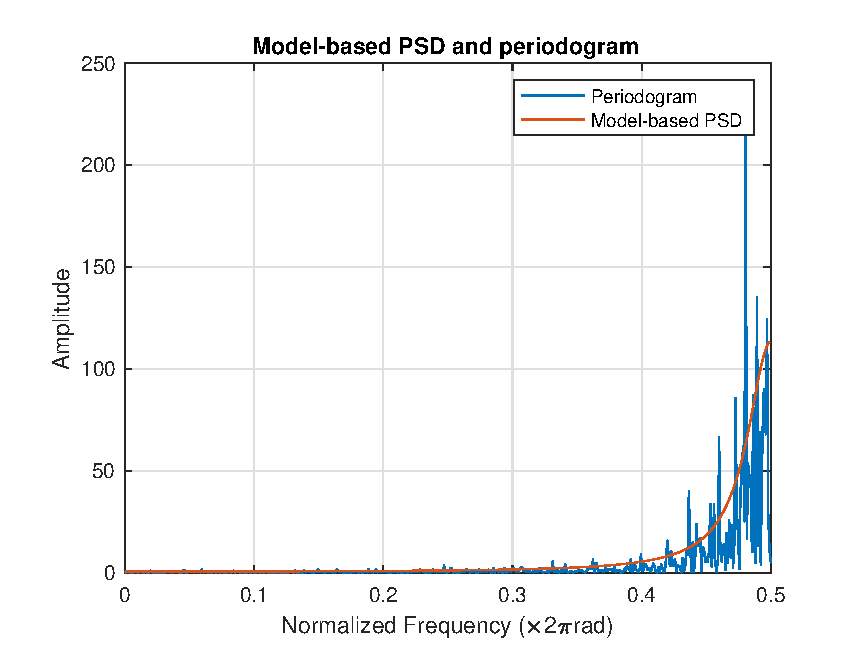
\includegraphics[width=7cm]{assignment3figs/mod_pgm.eps}
    \caption{Model-based PSD estimate vs periodogram.}
    \label{fig:mod_pgm}
\end{figure}

\noindent
This process was repeated using data from the Sunspot time series, both with the original and standardised data, varying model order. The results of this are shown in Figure \ref{fig:sunmodels}.

\begin{figure}[H]
    \centering
    \subfloat[Original Sunspot data.]{{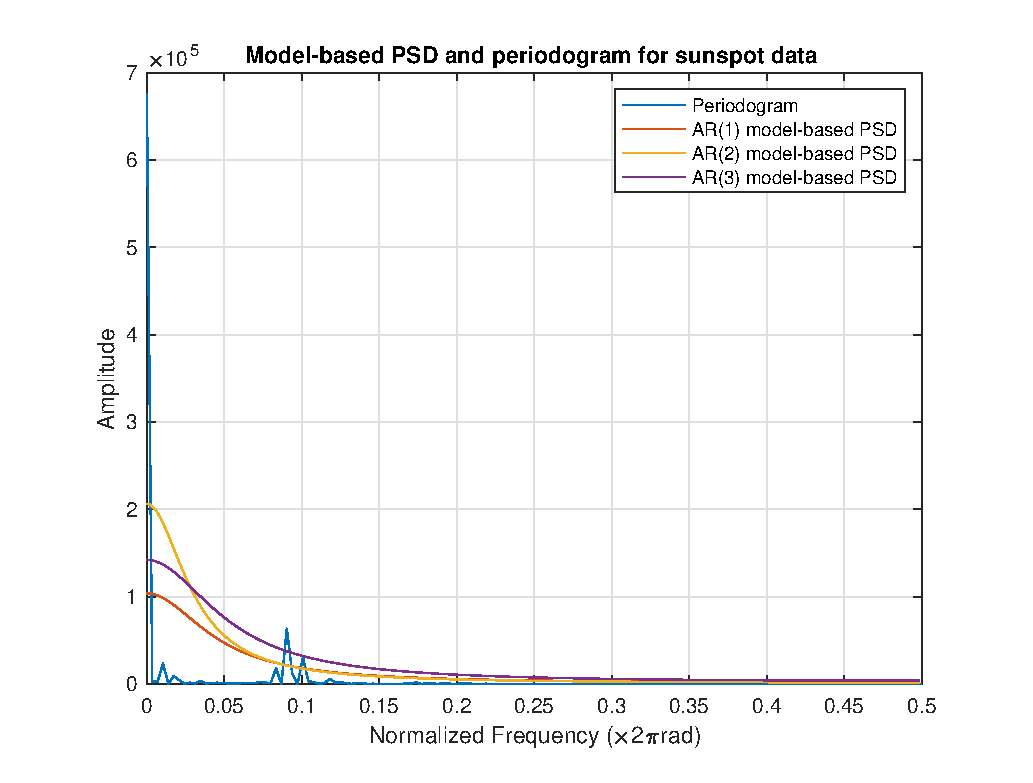
\includegraphics[width=7cm]{assignment3figs/pgm_mods_sun.eps}}}
    \subfloat[Standardised Sunspot data.]{{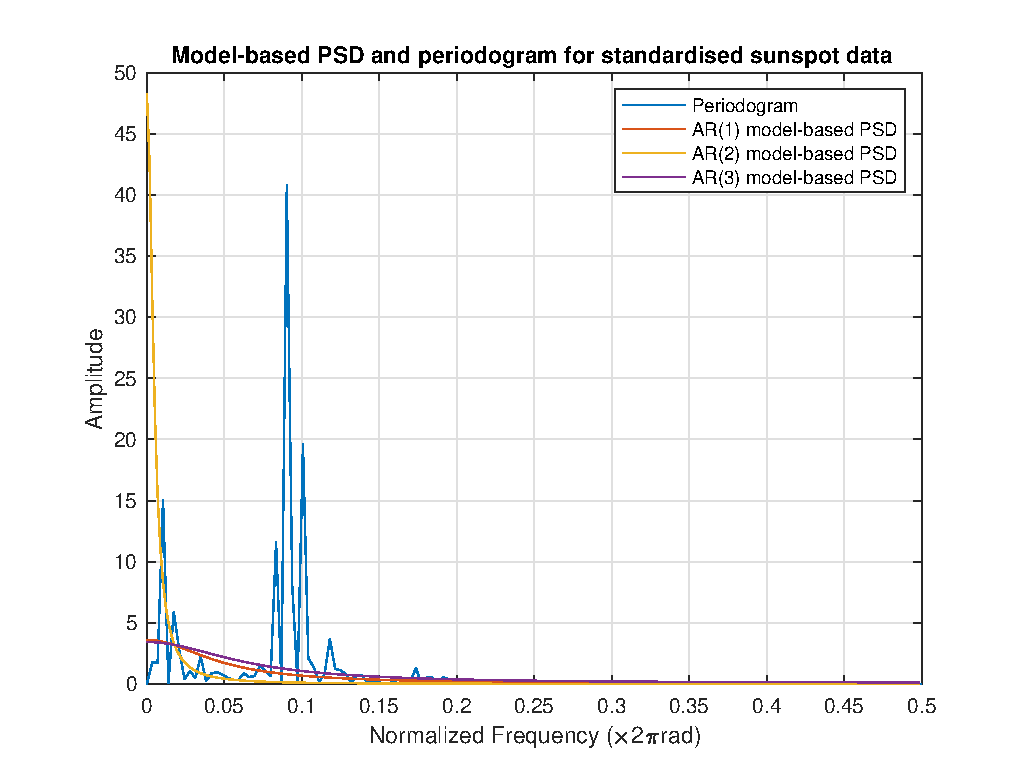
\includegraphics[width=7cm]{assignment3figs/stand.eps}}}
    \caption{Periodogram and model-based PSDs for Sunspot data.}
    \label{fig:sunmodels}
\end{figure}

\noindent
The model appears to be more accurate for the original Sunspot time series data, though none of the models appear to approximate the PSD well.

% 3.3 The Least Squares Estimation (LSE) of AR Coefficients
\subsection{The Least Squares Estimation (LSE) of AR Coefficients}

For an AR process given by Equation \ref{eqn:arproc}, the biased ACF can be calculated by Equation \ref{eqn:biasacf}.

\begin{equation}
x[n]=a_{1} x[n-1]+a_{2} x[n-2]+\cdots+a_{p} x[n-p]+w[n], \quad w[n] \sim \mathcal{N}(0,1)
\label{eqn:arproc}
\end{equation}

\begin{equation}
\hat{r}_{x x}[k]=\frac{1}{N} \sum_{n=0}^{N-1-k} x[n] x[n+k]
\label{eqn:biasacf}
\end{equation}

\noindent
For the process in Equation \ref{eqn:arproc}, this can be written as in Equation \ref{eqn:again}.

\begin{equation}
\hat{r}_{x x}[k]=\sum_{i=1}^{p} a_{i} \hat{r}_{x x}[k-i]+\epsilon[k], \quad \text { for } i \geq 1
\label{eqn:again}
\end{equation}

\noindent where $\epsilon[k]$ is the error due to the effect of errors on ACF estimate.

\subsubsection{Cost function}

The LS cost function for finding the unknown AR coefficients is given by Equation process \ref{eqn:cost}.

\begin{equation}
J=\sum_{k=1}^{M}\left[\hat{r}_{x x}[k]-\sum_{i=1}^{p} a_{i} \hat{r}_{x x}[k-i]\right]^{2}, \text { for } M \geq p
\label{eqn:cost}
\end{equation}

\noindent
Substituting Equation \ref{eqn:again} into \ref{eqn:cost}, Equation \ref{eqn:epsilon} is obtained.

\begin{equation}
J=\sum_{k=1}^{M} \epsilon[k]^{2}=\epsilon^{T} \epsilon
\label{eqn:epsilon}
\end{equation}

\noindent
This can be rewritten as below to obtain Equation \ref{eqn:epsilon2}.

\begin{equation}
J = (x-s)^{T}(x-s)
\label{eqn:epsilon2}
\end{equation}

\noindent
The signal model $\boldsymbol{s}$ is calculated as $\boldsymbol{s = Ha}$, therefore Equation \ref{eqn:epsilon2} can be rewritten as \ref{eqn:j}.

\begin{equation}
J=(x-\mathbf{H a})^{T}(x-\mathbf{H a})
\label{eqn:j}
\end{equation}

\noindent
where the observation matrix $\boldsymbol{H}$ is given by Equation \ref{eqn:obs}.

\begin{equation}
\mathbf{H}=\left[\begin{array}{cccc}
x[n-1] & x[n-2] & \dots & x[n-p] \\
x[n] & x[n-1] & \dots & x[n+1-p] \\
\vdots & \vdots & \vdots & \ddots \\
x[N-1] & x[N-2] & \dots & x[N-p]
\end{array}\right]
\label{eqn:obs}
\end{equation}


\subsubsection{The observation matrix H}

Since the signal x[n] is constant across realisations, $\boldsymbol{H}$ does not display any random behaviour and is therefore deterministic. 
% 3.4 Spectrogram for time-frequency analysis: dial tone pad
\subsection{Spectrogram for time-frequency analysis: dial tone pad}

\subsubsection{Randomly generated London landline number}

The underlying concept of touch-tone telephone dialling is the Dual Tone Multi-Frequency (DTMF) system which assigns a signal composed of two sinusoids to each button of the keypad. This is described by Equation \ref{eqn:dtmf}.

\begin{equation}
y[n]=\sin \left(2 \pi f_{1} n\right)+\sin \left(2 \pi f_{2} n\right)
\label{eqn:dtmf}
\end{equation}

\noindent
where $f_1$, $f_2$ are the frequencies in Hz, and n is the time index. The frequencies corresponding to each digit are shown in Table \ref{Tab:DTMF}.

\begin{table}[H]
\centering
\begin{tabular}{c|c|c|c} 
& $1209 \mathrm{Hz}$ & $1336 \mathrm{Hz}$ & $1477 \mathrm{Hz}$ \\
\hline $697 \mathrm{Hz}$ & $\mathbf{1}$ & $\mathbf{2}$ & $\mathbf{3}$ \\
\hline $770 \mathrm{Hz}$ & $\mathbf{4}$ & $\mathbf{5}$ & $\mathbf{6}$ \\
\hline $852 \mathrm{Hz}$ & $\mathbf{7}$ & $\mathbf{8}$ & $\mathbf{9}$ \\
\hline $941 \mathrm{Hz}$ & $*$ & $\mathbf{0}$ & $\#$
\end{tabular}
\caption{DTMF frequencies.}
\label{Tab:DTMF}
\end{table}


\noindent
Using the DTMF system outlined above, I generated a signal for the dial-tone sequence dialing randomly generated London land-line number. The number generated was '02049726813'.

\begin{figure}[H]
    \centering
    \subfloat[Full sequence.]{{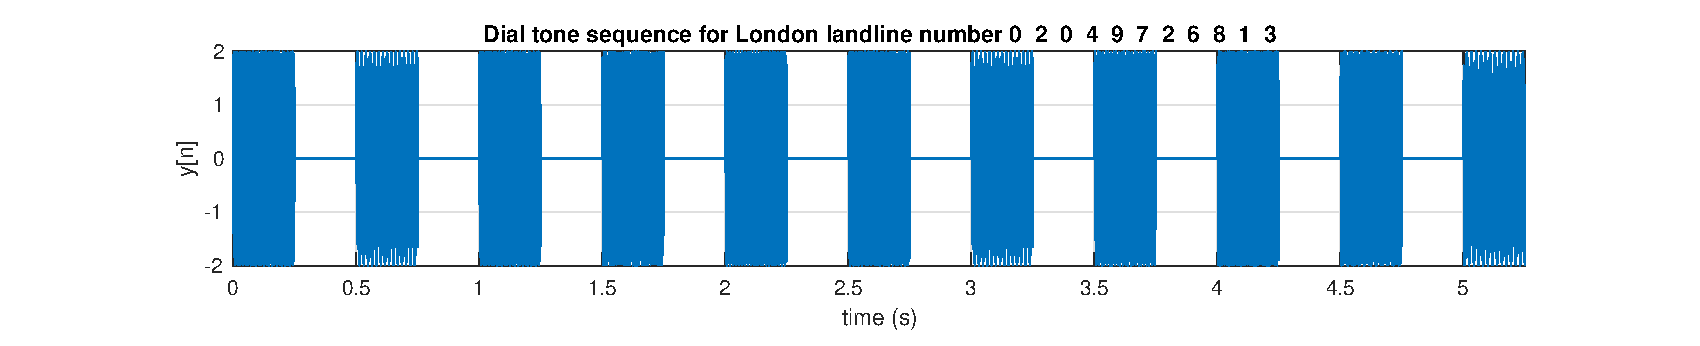
\includegraphics[width=18.5cm]{assignment3figs/tonesequence.eps}}}\\
    \subfloat[Zoomind in on digits '0' and '2'.]{{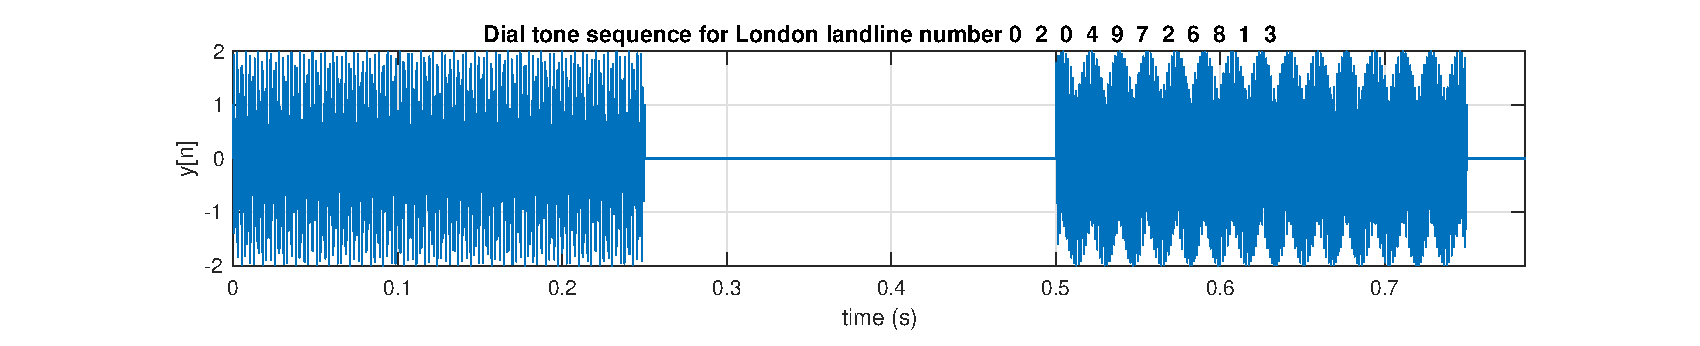
\includegraphics[width=18.5cm]{assignment3figs/tone02.eps}}}
    \caption{Signal for dial-tone sequence '02049726813'.}
    \label{fig:toneseqs}
\end{figure}

\noindent
The Nyquist frequency is 2954Hz since the maximum frequency used in the DTMF system is 1477Hz. A sampling frequency of 32768Hz ensures that there will be no aliasing for signals up to a frequency 16384Hz. This is significantly higher than required  but oversampling increases the SNR so should always be done if possible.

\subsubsection{Spectrogram and magnitude spectra}

A spectrogram was generated for this dial-tone sequence using MATLAB's \code{spectrogram()} function, and it shown in Figure \ref{fig:spec}.

\begin{figure}[H]
    \centering
    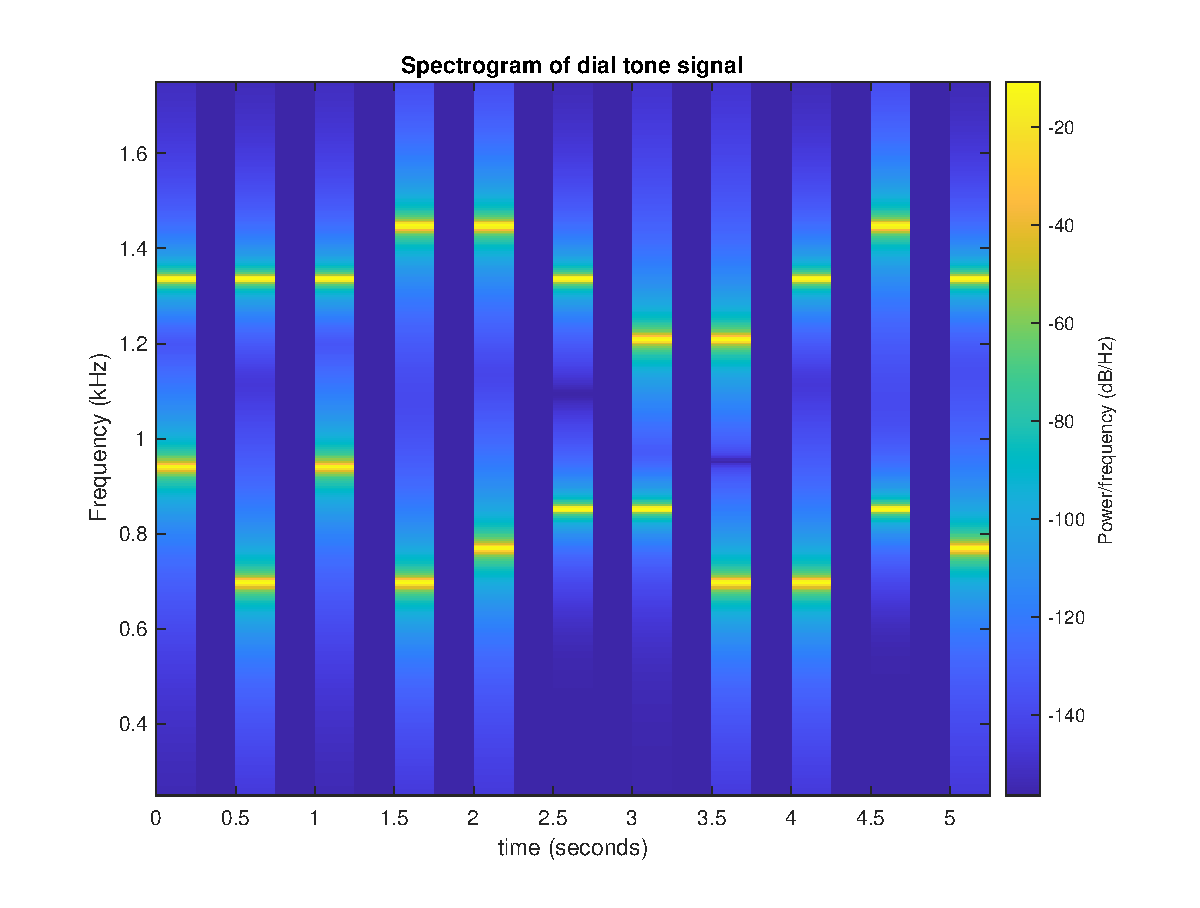
\includegraphics[width=12cm]{assignment3figs/spec1.eps}
    \caption{Spectrogram of dial-tone sequence.}
    \label{fig:spec}
\end{figure}

\noindent
This spectrogram clearly shows peaks in signal power for two distinct frequencies for each digit dialed. Checking these against the values in the table provided that describes the DTMF system, the peaks correspond to the expected values. These peaks can be revealed more clear by magnitude spectra, as shown in Figure \ref{fig:magspec}.

\begin{figure}[H]
    \centering
    \subfloat[Full sequence.]{{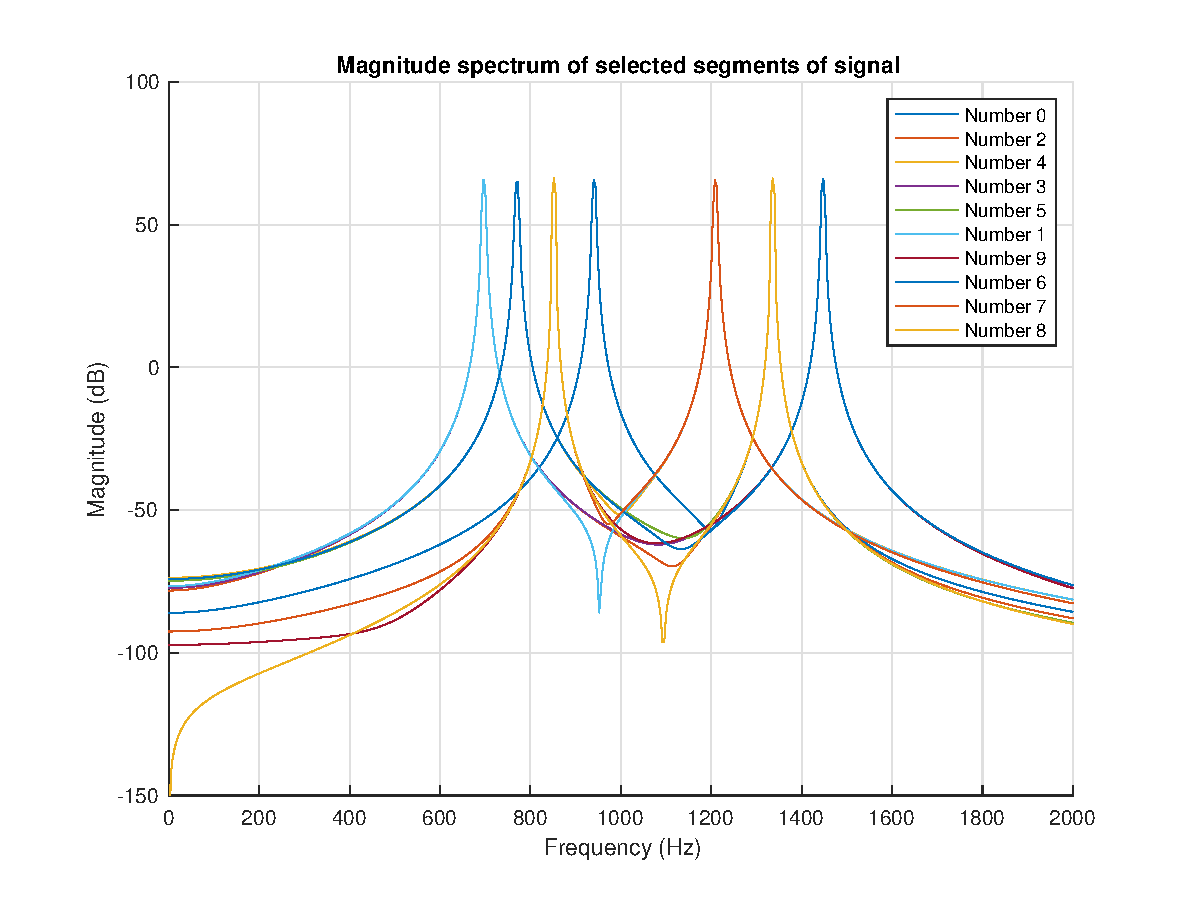
\includegraphics[width=8.5cm]{assignment3figs/magspec_all.eps}}}
    \subfloat[Isolated '0' and '2' digits.]{{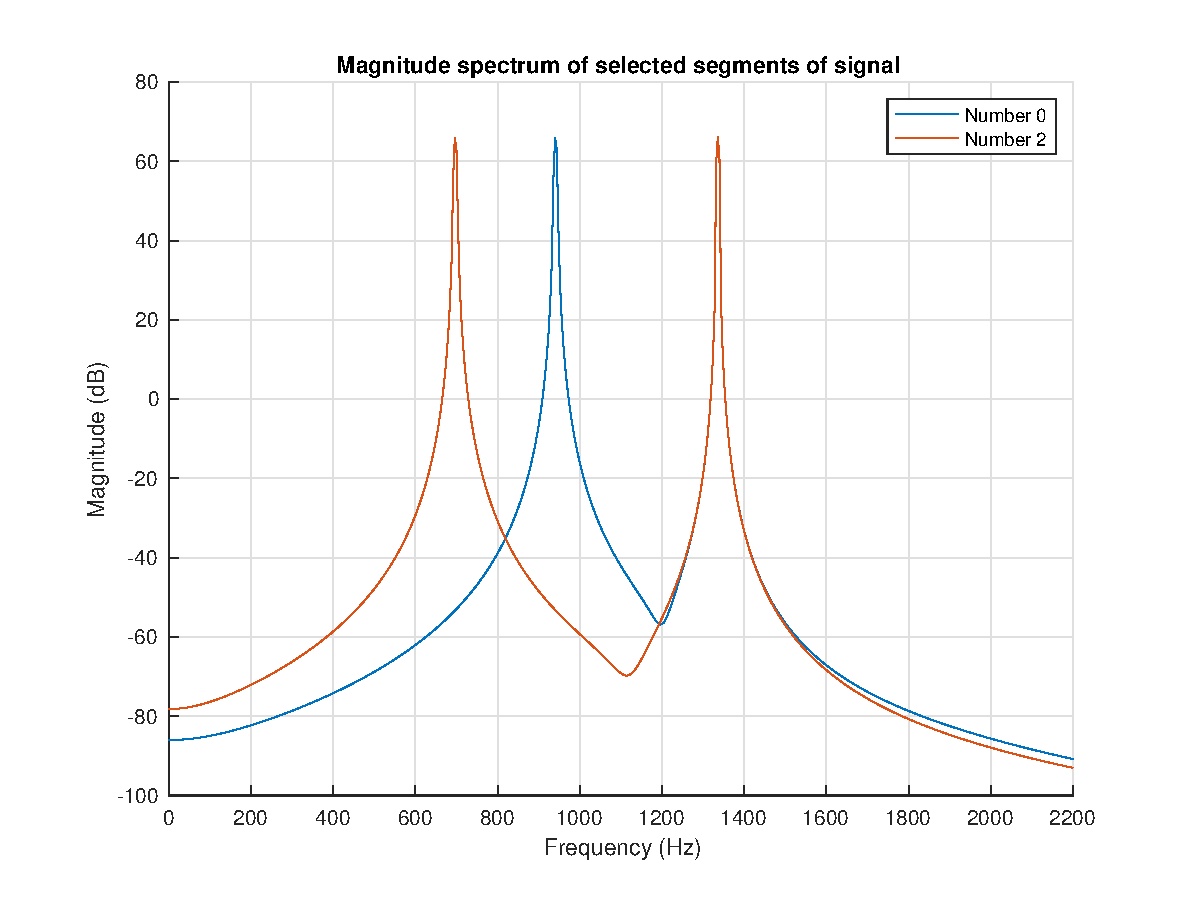
\includegraphics[width=8.5cm]{assignment3figs/magspec.eps}}}
    \caption{Magnitude spectra for dial sequence signal.}
    \label{fig:magspec}
\end{figure}

\noindent
In Figure \ref{fig:magspec}a, there are 7 distinct peaks which correspond to the seven frequencies which make up the tones for all digits in the DTMF system. Isolating the digits '0' and '2' as in Figure \ref{fig:magspec}b, there are 3 distinct peaks which correspond the three distinct frequencies that make up the tones for these two digits.

\subsubsection{Key Classification}

Looking at the spectrogram in Figure \ref{fig:spec} and Table \ref{Tab:DTMF}, it is possible to identify the keys which have been pressed as well as their order. If the magnitude spectra in Figure \ref{fig:magspec} are available, but not the spectrogram, then it is possible to identify the keys which have been pressed, but not the order in which they have been pressed. This is because a magnitude spectrum encapsulates no time-domain information. 

\subsubsection{Introducing channel noise}

In order to better simulate real-world conditions, WGN noise of increasing variance was introduced to corrupt the dial-tone sequence signal. The corrupted signals are shown in Figure \ref{fig:noisy}, along with their spectrograms and magnitude spectra.

\begin{figure}[H]
\begin{subfigure}{.32\textwidth}
  \centering
  \includegraphics[width=\linewidth]{assignment3figs/sig_sd01.eps}  
  \caption{Corrupted signal, $\sigma_{n}^{2} = 0.01$.}
\end{subfigure}
\begin{subfigure}{.32\textwidth}
  \centering
  \includegraphics[width=\linewidth]{assignment3figs/spec_sd01.eps}  
  \caption{Spectrogram, $\sigma_{n}^{2} = 0.01$.}
\end{subfigure}
\begin{subfigure}{.32\textwidth}
  \centering
  \includegraphics[width=\linewidth]{assignment3figs/magspec_sd01.eps}  
  \caption{Magnitude spectrum, $\sigma_{n}^{2} = 0.01$.}
\end{subfigure}\\
\begin{subfigure}{.32\textwidth}
  \centering
  \includegraphics[width=\linewidth]{assignment3figs/sig_sd1.eps}  
  \caption{Corrupted signal, $\sigma_{n}^{2} = 1$.}
\end{subfigure}
\begin{subfigure}{.32\textwidth}
  \centering
  \includegraphics[width=\linewidth]{assignment3figs/spec_sd1.eps}  
  \caption{Spectrogram, $\sigma_{n}^{2} = 1$.}
\end{subfigure}
\begin{subfigure}{.32\textwidth}
  \centering
  \includegraphics[width=\linewidth]{assignment3figs/magspec_sd1.eps}  
  \caption{Magnitude spectrum, $\sigma_{n}^{2} = 1$.}
\end{subfigure}\\
\begin{subfigure}{.32\textwidth}
  \centering
  \includegraphics[width=\linewidth]{assignment3figs/sig_sd10.eps}  
  \caption{Corrupted signal, $\sigma_{n}^{2} = 100$.}
\end{subfigure}
\begin{subfigure}{.32\textwidth}
  \centering
  \includegraphics[width=\linewidth]{assignment3figs/spec_sd10.eps}  
  \caption{Spectrogram, $\sigma_{n}^{2} = 100$.}
\end{subfigure}
\begin{subfigure}{.32\textwidth}
  \centering
  \includegraphics[width=\linewidth]{assignment3figs/magspec_sd10.eps}  
  \caption{Magnitude spectrum, $\sigma_{n}^{2} = 100$.}
\end{subfigure}
\caption{Corrupted dial-tone sequence signals with their spectrograms and magnitude spectra.}
\label{fig:noisy}
\end{figure}

\noindent
It is qualitatively obvious that introducing noise corrupts the signal from the left column of Figure \ref{fig:noisy}. To gain a more quantitative insight into the nature of this corruption, the spectrograms in the middle column are useful. When the noise
variance $\sigma_{n}^{2}$ = 0.01, the power peaks are still easily distinguishable. For $\sigma_{n}^{2}$ = 1, they are less clear but still identifiable. However, when $\sigma_{n}^{2}$ = 100, the SNR is so low that the noise power is roughly equivalent to the signal power and the peaks of the tone frequencies are no longer distinguishable. The magnitude spectra prove more useful for identifying tone frequencies in the noisy signal. The tone frequencies are identifiable from the maxima of the magnitude spectra even for noise variance $\sigma_{n}^{2}$ = 100 (Figure \ref{fig:noisy}i). It is important to note that these magnitude spectra are only for the digits '0' and '2', so whilst the three frequencies for these digits alone are identifiable, the magnitude spectra for the full sequence may be less clear and it may not be possible to identify all tone frequencies.


% 3.5 Real world signals: Respiratory sinus arrhythmia from RR-Intervals
\subsection{Real world signals: Respiratory sinus arrhythmia from RR-Intervals}

The periodogram was calculated for the RRI signals for the three trials from the iAmp experiment. This was both for the original data and for data windowed with window lengths of 50 and 150 and averaged across periodograms. The results are shown in Figure \ref{fig:RRIspecs}.

\begin{figure}[H]
\begin{subfigure}{.32\textwidth}
  \centering
  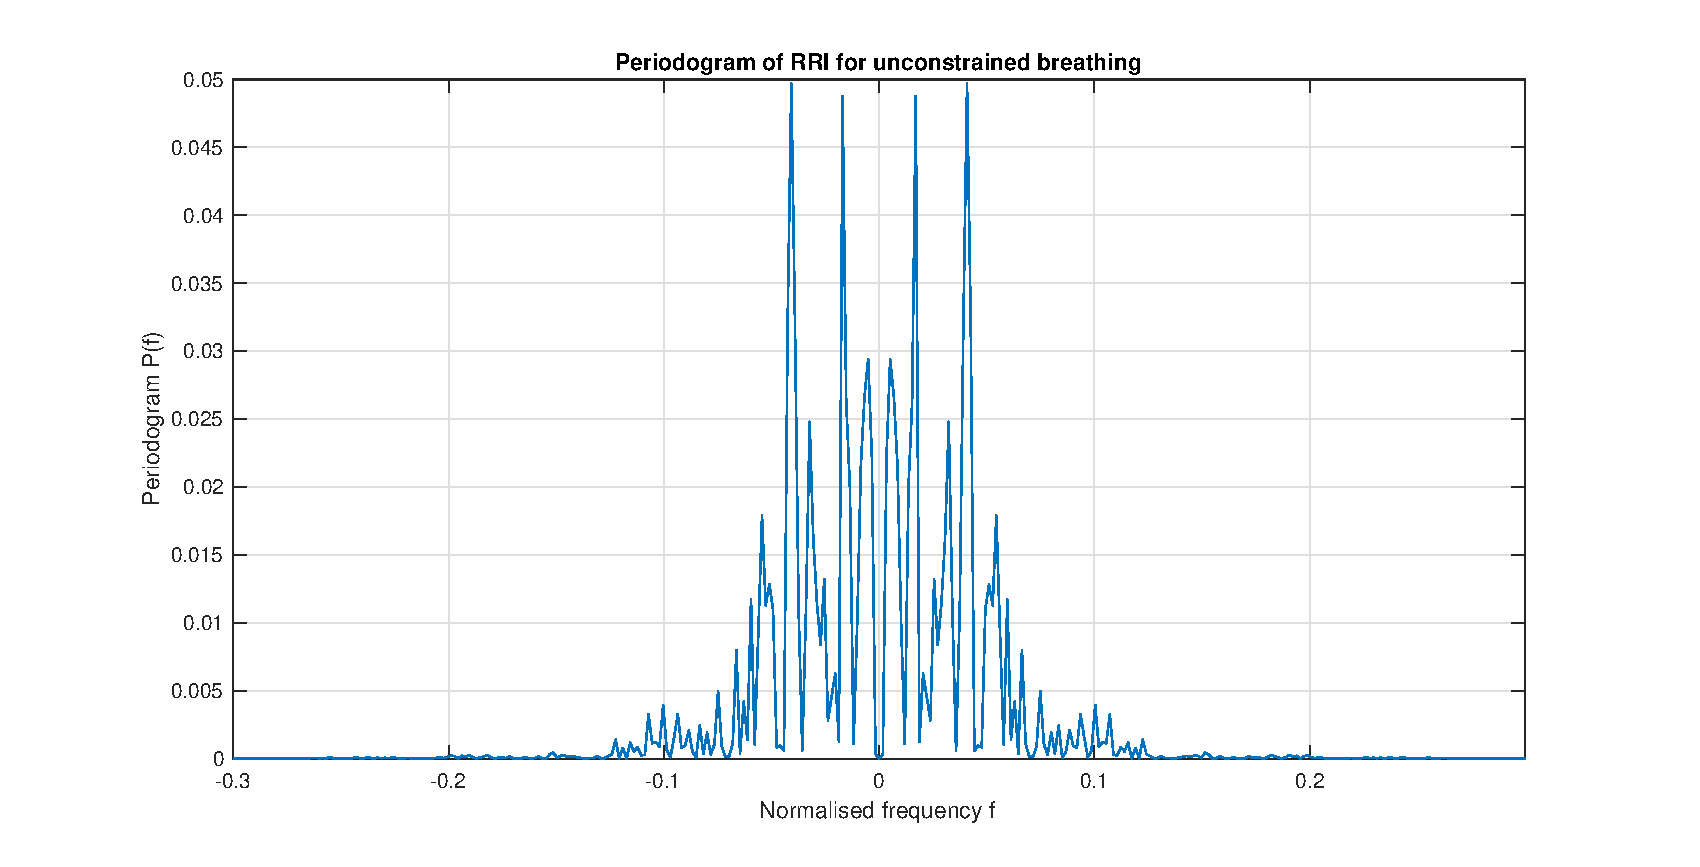
\includegraphics[width=\linewidth]{assignment3figs/new_pgm_uncon_noave.eps}  
  \caption{Trial 1.}
\end{subfigure}
\begin{subfigure}{.32\textwidth}
  \centering
  \includegraphics[width=\linewidth]{assignment3figs/new_pgm_uncon_ave50.eps}  
  \caption{Trial 1, averaged with window 50.}
\end{subfigure}
\begin{subfigure}{.32\textwidth}
  \centering
  \includegraphics[width=\linewidth]{assignment3figs/new_pgm_uncon_ave150.eps}  
  \caption{Trial 1, averaged with window 150.}
\end{subfigure}\\
\begin{subfigure}{.32\textwidth}
  \centering
  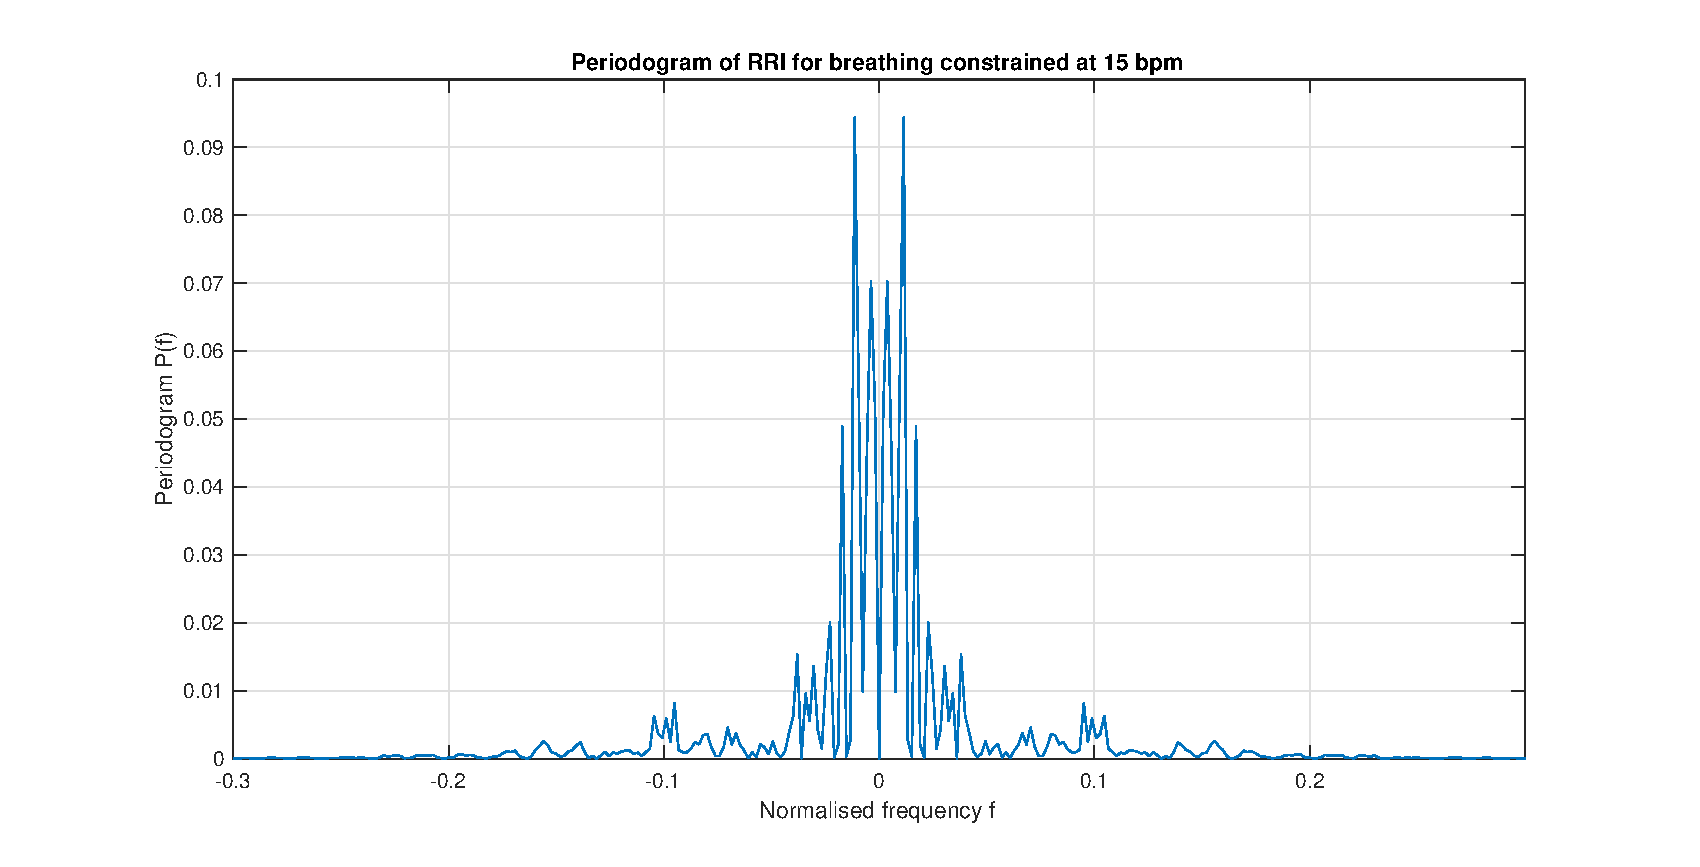
\includegraphics[width=\linewidth]{assignment3figs/new_pgm_con15_noave.eps}
  \caption{Trial 2.}
\end{subfigure}
\begin{subfigure}{.32\textwidth}
  \centering
  \includegraphics[width=\linewidth]{assignment3figs/new_pgm_con15_ave50.eps}  
  \caption{Trial 2, averaged with window 50.}
\end{subfigure}
\begin{subfigure}{.32\textwidth}
  \centering
  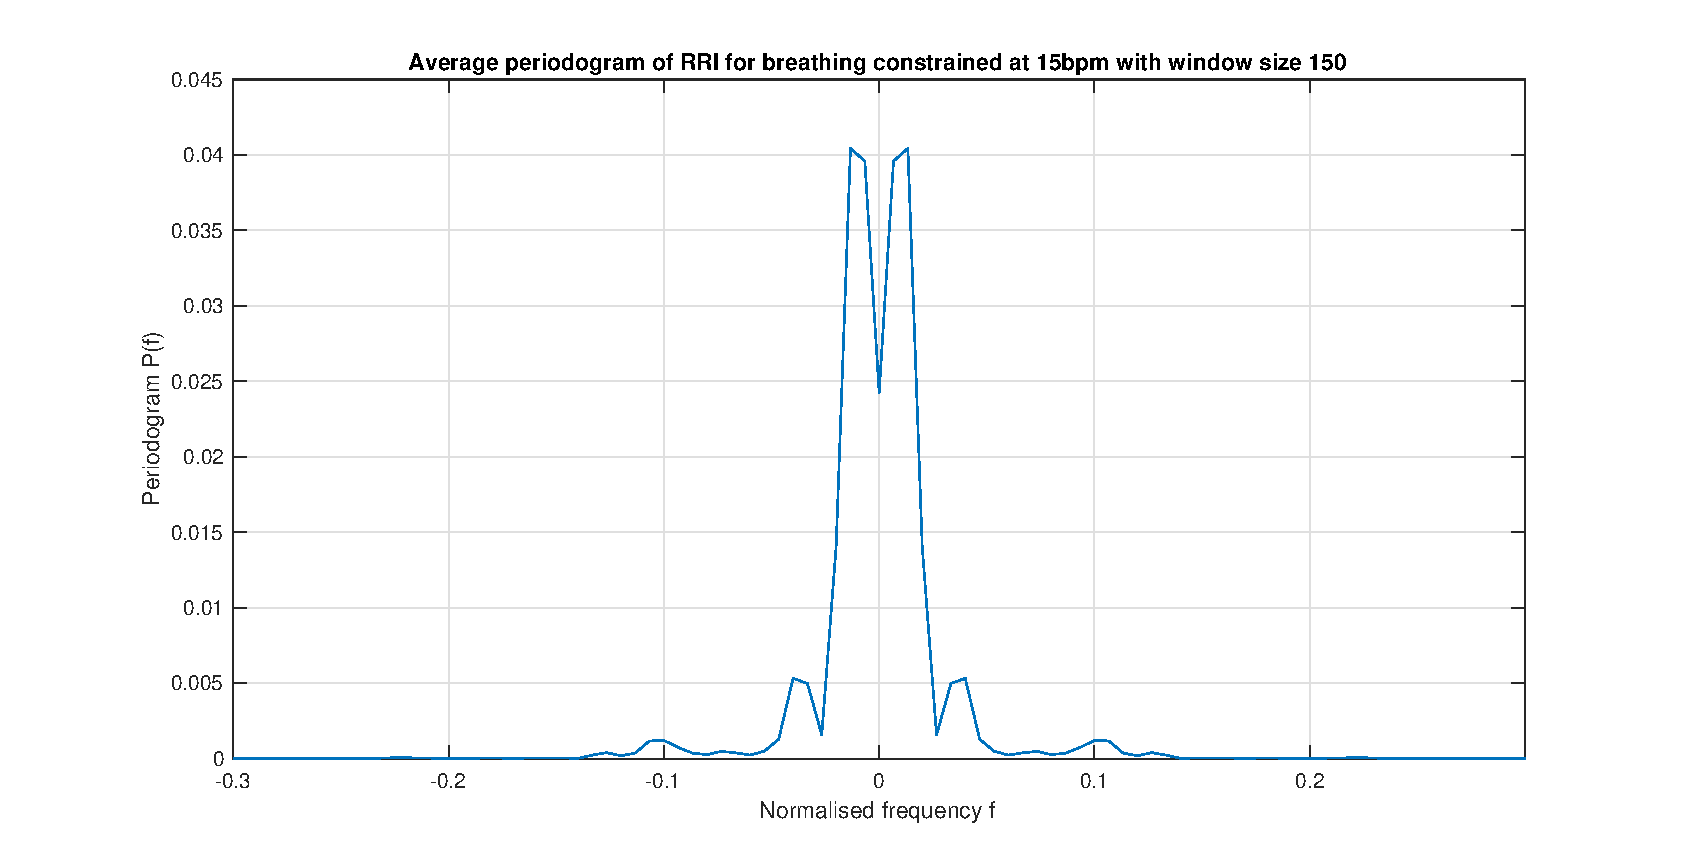
\includegraphics[width=\linewidth]{assignment3figs/new_pgm_con15_ave150.eps}  
  \caption{Trial 2, averaged with window 150.}
\end{subfigure}\\
\begin{subfigure}{.32\textwidth}
  \centering
  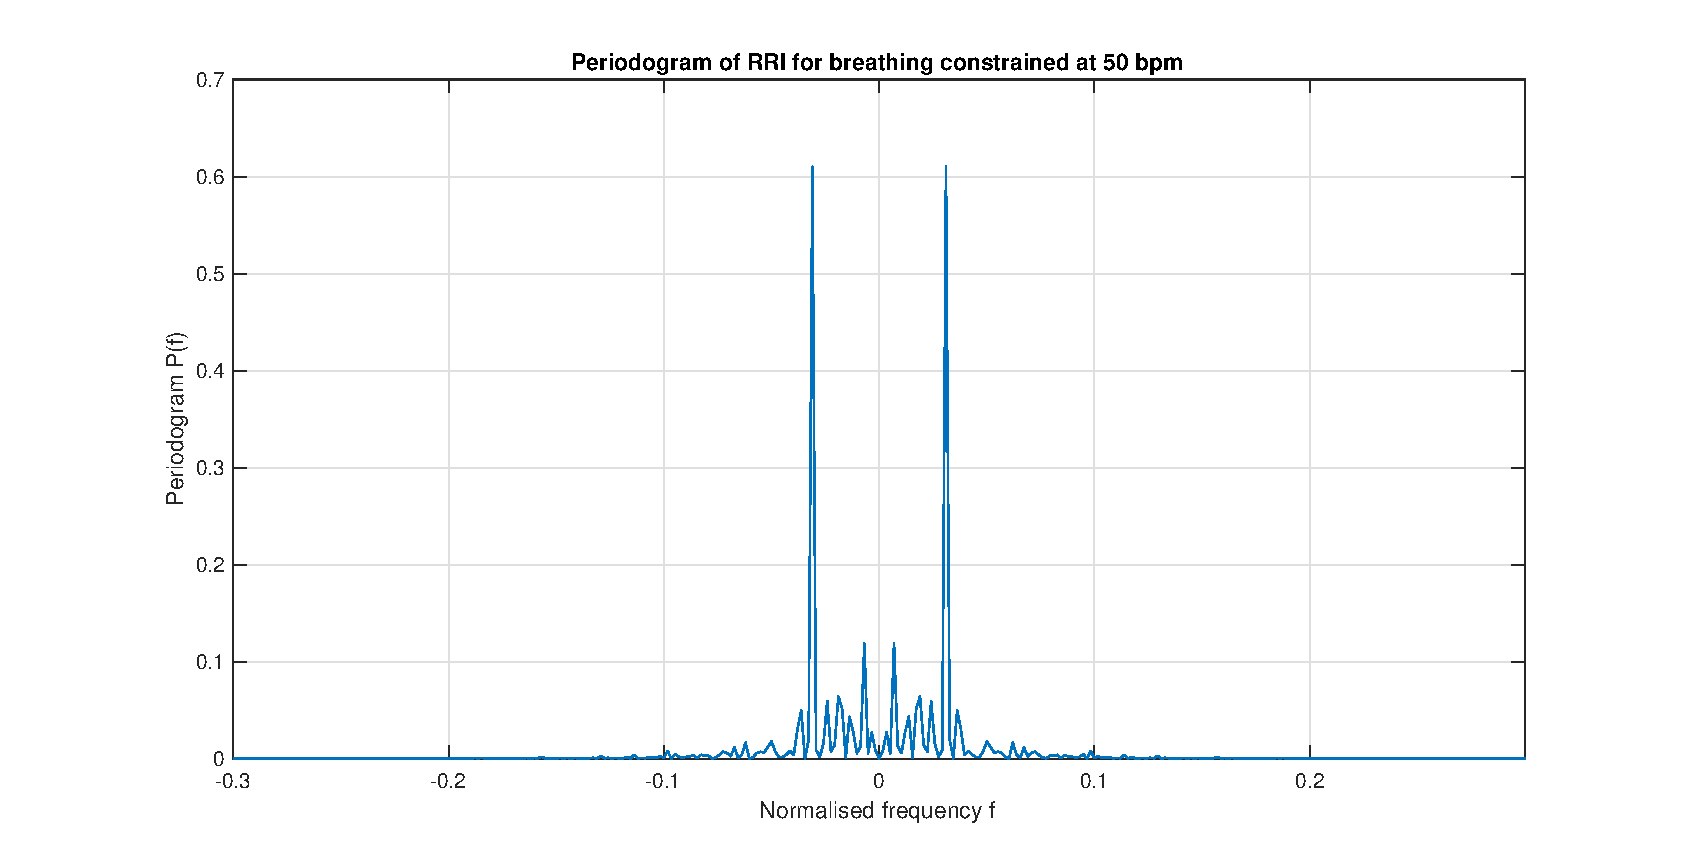
\includegraphics[width=\linewidth]{assignment3figs/new_pgmcon50_noave.eps}
  \caption{Trial 3.}
\end{subfigure}
\begin{subfigure}{.32\textwidth}
  \centering
  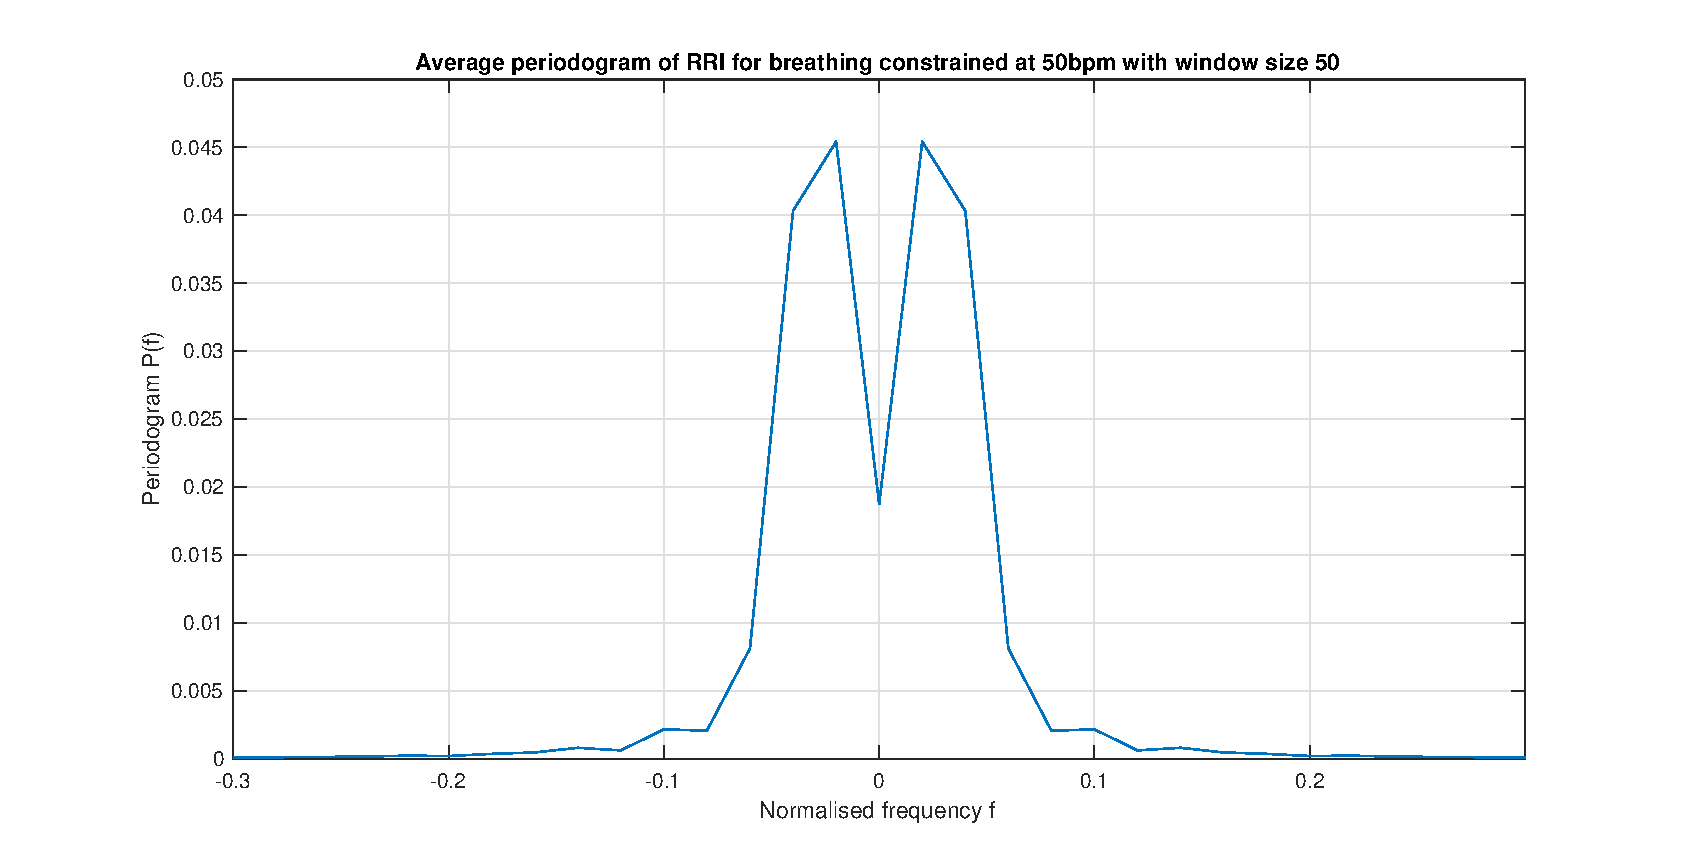
\includegraphics[width=\linewidth]{assignment3figs/new_pgm_con50_ave50.eps}  
  \caption{Trial 2, averaged with window 50.}
\end{subfigure}
\begin{subfigure}{.32\textwidth}
  \centering
  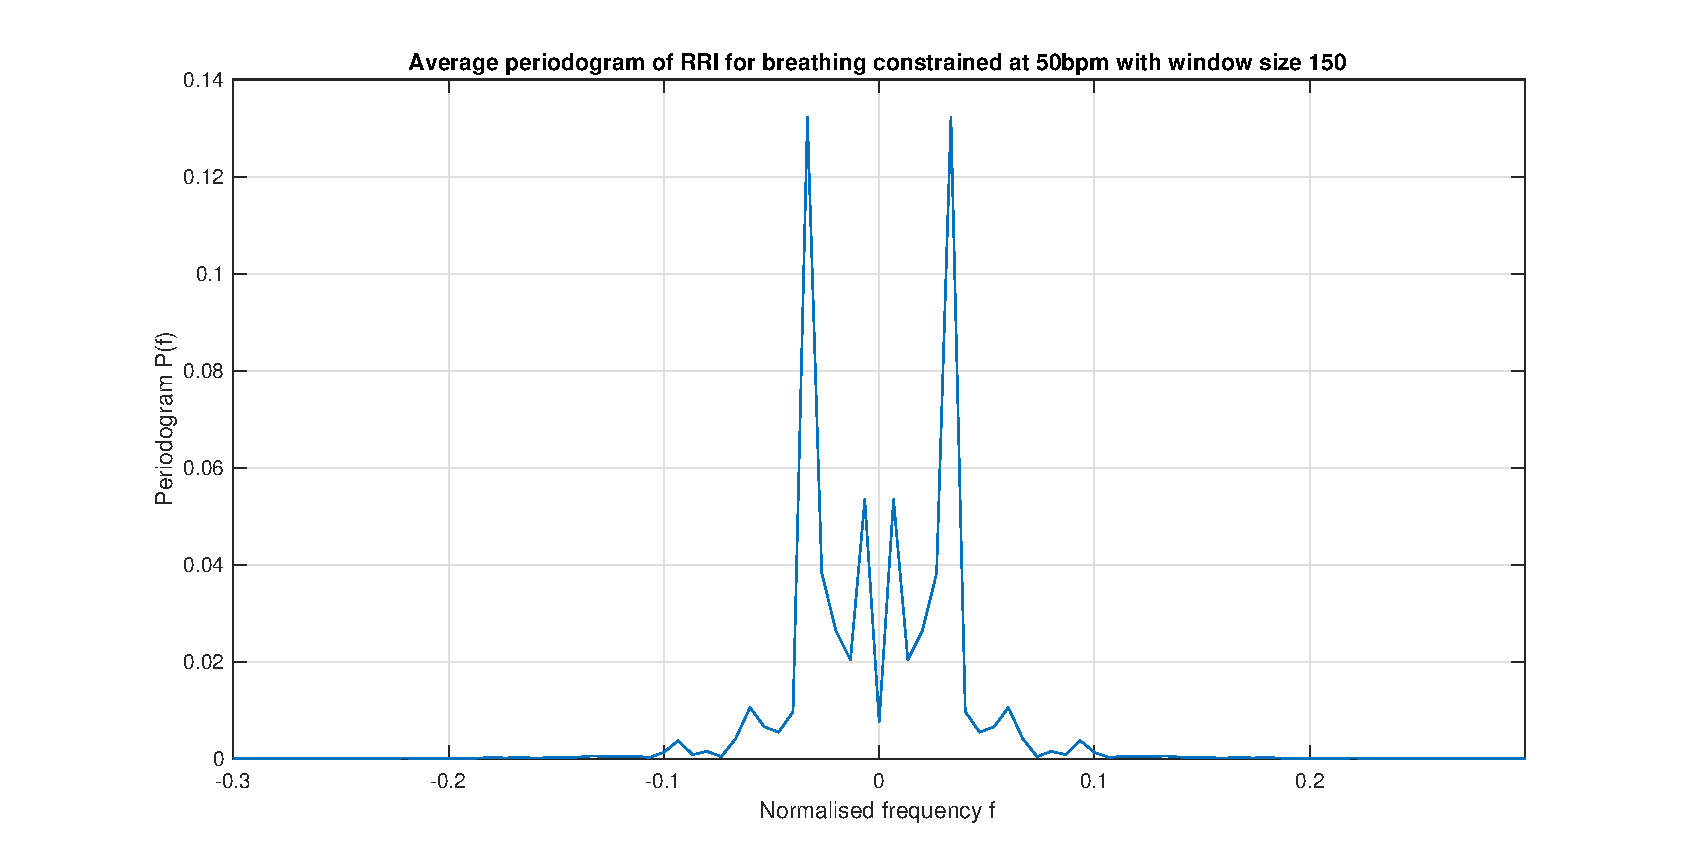
\includegraphics[width=\linewidth]{assignment3figs/new_pgm_con50_ave150.eps}  
  \caption{Trial 2, averaged with window 150.}
\end{subfigure}
\caption{Periodograms for all trials of RRI signals with different windowing applied.}
\label{fig:RRIspecs}
\end{figure}

\noindent
It is apparent from the left column of Figure \ref{fig:RRIspecs} that each of the trials have peaks at different normalised frequencies. This shows that the dominant frequencies in each signal (which should  be indicative of heart rate) are different, suggesting that RSA (whereby altering breathing rate has an effect on heart rate) does take place. Windowing and averaging has the effect of smoothing the periodogram, with more prominent smoothing taking place for the shorter window size of 50 (middle column of Figure \ref{fig:RRIspecs}). This can be explained by the inverse relationship of time and frequency. The signals averaged using window length 150 (right column of Figure \ref{fig:RRIspecs} are the most useful for deducing the dominant frequencies in each trial. Trial 1 has a dominant peak at a normalised frequency of 0.04, Trial 2 at 0.02 and Trial 3 at 0.03. Trial 1 has a second peak at 0.02, Trial 2 at 0.04 and Trial 3 at 0.01 During RSA, the heart rate increases slightly during inspiration and decreases slighty during exhalation. Therefore, the two peaks seen in each spectrogram correspond to the heart rates during inspiration and exhalation for each exercise.